% Temporarily as a seperate document
% Will be placed inside the IROS root latex file

\documentclass[10pt,a4paper]{article}
\usepackage[latin1]{inputenc}
\usepackage{amsmath}
\usepackage{amsthm}
\usepackage{amsfonts}
\usepackage{amssymb}
\usepackage{mathtools}
\usepackage{graphicx}
\usepackage{color}

% theorem environment
\newtheorem{prop}{Proposition}[section]
\newtheorem{theorem}{Theorem}[section]
\newtheorem{prop2}{Proposition}
\newtheorem{lem}{Lemma}
\newtheorem{ex}{Example}

% custom commands
\newcommand\at[2]{\left.#1\right|_{#2}} % the at differential sign
\newcommand\scalemath[2]{\scalebox{#1}{\mbox{\ensuremath{\displaystyle #2}}}} % scaling matrices

%% custom macros
\newcommand{\todo}{\textcolor{red}{TODO}} % TODO!
\newcommand{\kin}{\mathcal{T}} % used to denote inverse kinematics
\newcommand{\invKin}{\mathcal{T}^{-1}} % used to denote inverse kinematics

\newcommand{\joint}{q} % used to denote robot state in joint space
\newcommand{\state}{\bar{\joint}} % denotes the generalized coordinates - joint space and velocity coordinates
\newcommand{\dmp}{s} % used to denote the dmp trajectory states
\newcommand{\error}{e} % difference between state and reference
\newcommand{\traj}{r} % used to denote the points on the trajectory to be tracked

\newcommand{\dist}{\epsilon} % denotes the disturbances acting on the rigid body dynamics
\newcommand{\linDist}{d} % denotes the disturbances on the LTV model

\newcommand{\sysInput}{u} % used to denote the system inputs
\newcommand{\linInput}{\tilde{u}} % denotes the LTV inputs
\newcommand{\trjInput}{\nu} % denotes the inputs on the trajectory


% % % % DMP terminology % % % %
\newcommand{\fullvec}{\psi} % full vector for state-ref-dmp-goal
\newcommand{\force}{f} % forcing term of the dmps
\newcommand{\phase}{x} % phase of the dmp
\newcommand{\weights}{w} % weights of the dmp
\newcommand{\basis}{\Phi} % basis functions of the dmp as a matrix

% % % % ILC terminology % % % %
\newcommand{\qmatrix}{\Gamma} % denotes the filtering qmatrix term of Bristow et al.
\newcommand{\lmatrix}{L} % denotes the learning matrix of Bristow et al.

\newcommand{\observations}{\mathbf{y}} % used for the observed output
\newcommand{\dynamics}{f}
\newcommand{\dynamicsNominal}{f_{\mathrm{nom}}}
\newcommand{\policy}{\mathbf{\pi}}
\newcommand{\ValueFunction}{J}
\newcommand{\episode}{k} % used for episode number

\newcommand{\totalTime}{T} % total time duration 
\newcommand{\numSteps}{N} % total number of time steps
\newcommand{\numepisode}{K} % total number of episodes

\newcommand{\threshold}{\epsilon_s}
\newcommand{\alg}{\emph{wILC}}
\newcommand{\dataset}{E}

% Set the paths where all figures are taken from:
\graphicspath{{Pictures/}}
\mathtoolsset{showonlyrefs} 
\newcommand{\includesvg}[1]{%
% \executeiffilenewer{#1.svg}{#1.pdf}%
% {inkscape -z -D --file=#1.svg %
% --export-pdf=#1.pdf --export-latex}%
 \input{#1.pdf_tex}%
}

\author{Okan Ko\c c}
\title{Optimal Striking Movement Representation \& Execution}
\begin{document}
\maketitle

\section{Introduction}

% fill missing citations

Most reaching tasks in control and robotics can be phrased as \emph{tracking} problems, where the dynamical system needs to follow a certain predefined trajectory in order to reach the goal state. 

Robotic table tennis in particular consists of planning, generating and executing a series of such (episodic) single stroke trajectories. These trajectories need to be followed very closely with motor commands in practice, in order to return the ball to the desired positions. 

% maybe cite Jens' review paper
There have been many attempts in the reinforcement learning \cite{Sutton98} and control literature to learn to track these trajectories directly. Value function based methods take advantage of duality to solve the Bellman's equation but suffer from the initial bias or representation in estimating the value function. Policy search methods directly solve the Bellman's equation in a parameterized policy space and can be much more effective in practice (in robotics). 

Episodic policy search methods 

Approximation and control errors in table tennis make the application of DMPs less useful in practice. Small changes to DMPs can often make them more useful.

Gait patterns often cause upper body oscillations, which break gait tracking. Can we adapt gait DMPs to facilitate the execution?

The research question that we tackle in this article consists of the following:

\begin{itemize}
\item How can we generate optimally hitting Dynamic Movement Primitives (DMPs)?

\item When we have modelling inaccuracies, how can we create a DMP $\dmp(t)$ such that the robot executes the desired hitting motion?
\end{itemize}

Finally our contributions can be summarized as follows:

\begin{itemize}
\item We form a link between the Iterative Learning Control literature and policy gradient based policy search approaches in Reinforcement Learning and develop a new algorithm that feeds on the strengths of both domains.

\item We form the first coherent framework where some of the biggest advantages of using Dynamic Movement Primitives are leveraged in the feedforward update rule.

\item On the theoretical side, we come up with a new ILC algorithm that is shown to be stable and monotonically convergent.
\end{itemize}

% Optimal Striking
% Talk about reinforcement learning
% Episodic setup - 'motor task consisting of a single stroke'
% Policy search methods
% DMPs
% Jens says : Dmps are a time-variant policy representation as they have an internal phase which corresponds to a clock with additional flexibility
% (e.g., for incorporating coupling effects, perceptual influences, etc.)
% Adapting DMPs
% Gait tracking
% Advantages of ILC Framework over Policy search 

\section{Related Work}

% missing citations
Dynamic Motor Primitives are a kind of kinematic policy representation that leverages the dynamical systems approach to modify the spring dynamics with a forcing term that enables it to mimic an executed trajectory. They include an internal phase or clock that ensures the convergence of the motor primitive to a desired goal state \cite{Ijspeert13}, \cite{Schaal07}. 

% Taken from the bimanual article
%They can be used to imitate or generate discrete and periodic trajectories, which can be modulated in various ways.

% Policy search methods
Policy search methods that modify the parameters of a DMP appeared first with the \emph{POWER} algorithm \cite{Kober08}.
% is this true?

Iterative Learning Control started out in the 1980s with the work of Arimoto et al. \cite{Arimoto84} as one of the first to define the genre with the PD-type update law \cite{Bristow06}. Monotonic convergence and stability guarantees are of central importance for the practical usefulness of ILC algorithms. They are shown for example in \cite{Bristow06}, \cite{Norrloef02}, \cite{Lee97}, \cite{Longman2000}.
% check these refs

% ILC work - mention Angela's work
As an example of a more sophisticated method than the PD-type update laws, Schoellig et al. \cite{Schoellig12} applied a Kalman-filter based convex optimization rule in the framework of ILC and showed its performance in quadrocopter flight.

% DMPs using Iterative Learning Control
DMPs have been also combined in a bimanual robotics task with ILC \cite{Gams13} where force feedback is used to enable compliant interaction with objects in an unknown enviornment. ILC is here used to learn a coupling term between the two arm trajectories. 
% used to modulate the DMP and learn ...


\section{Problem Statement}

Goal: Track a reference trajectory $\traj(t), \ 0 \leq t \leq T \ $ by applying the control inputs $\sysInput(t)$.

% this section probably belongs to a journal
\subsection{ILC Review}

In this section we will first review some of the results from the Iterative Learning Control (ILC) literature \cite{Bristow06}. Consider the nonlinear robot dynamics of the form:

\begin{equation}
\begin{aligned}
\ddot{\joint} &= \dynamics(\joint,\dot{\joint},\sysInput) + \dist(\joint,\dot{\joint})\\
\ddot{\joint} &= M^{-1}(\joint)\{ \tau(\sysInput) - C(\joint,\dot{\joint})\dot{\joint} - G(\joint)\} + \dist(\joint,\dot{\joint})\\
\end{aligned}
\label{dynamics}
\end{equation}

where on the right hand side are the terms due to the rigid body dynamics model and $\dist(\joint,\dot{\joint})$ are the (unmodeled) disturbances that act on the robot, such as viscous friction, stiction, etc. This system can be linearized around a given joint space trajectory $\traj(t), \ 0 \leq t \leq T$ with nominal inputs $\nu(t)$~\footnote{Nominal inputs $\sysInput_{\text{IDM}} = \nu(t)$ can be calculated using the inverse dynamics model.} to obtain the following linear time varying (LTV) representation:

\begin{equation}
\begin{aligned}
\dot{\error} = A(t)\error(t) + B(t)\linInput(t) + \linDist(t,\sysInput)
\end{aligned}
\label{LTV}
\end{equation}

where $\error(t) = \state(t) - \traj(t)$, $\state = [\joint,\dot{\joint}]^{\mathrm{T}}$, $\linInput(t) = \sysInput(t) - \trjInput(t)$ and the time varying matrices are:

\begin{equation}
\begin{aligned}
A(t) &= \at{\frac{\partial{\dynamics}}{\partial{\state}}}{(\traj(t),\trjInput(t))} \\
B(t) &= \at{\frac{\partial{\dynamics}}{\partial{\sysInput}}}{(\traj(t),\trjInput(t))}
\end{aligned}
\label{LTVmatrices}
\end{equation}

Here the additional term $\linDist(t,\sysInput)$ are due to the disturbances and the effects of the linearization. We can discretize (\ref{LTV}-\ref{LTVmatrices}) with step size $\Delta t$, $N = T/\Delta$ and step index $j = 1, \ldots, N$ to get the following discrete linear system:

\begin{equation}
\begin{aligned}
\error(j+1) = A^{D}(j)\error(j) + B^{D}(j)\linInput(j) + \linDist(j, \sysInput(1), \ldots, \sysInput(j))
\end{aligned}
\label{discreteLTV}
\end{equation}

Here $A^D$ and $B^D$ are the discretizations of \eqref{LTVmatrices} can be calculated using the trick \cite{Schoellig12}:

\begin{equation}
\begin{aligned}
\exp^{h
\left[
\scalemath{0.5}{
\begin{array}{c|c}
A(j) & B(j) \\ \hline
0 & 0
\end{array}}\right]}
&= 
\left[
\begin{array}{c|c}
A^{D}(j) & B^{D}(j) \\ \hline
0 & I
\end{array}\right] 
\end{aligned}
\label{discreteMatrices}
\end{equation}

We can stack these matrices together to get the following lifted-vector representation \cite{Bristow06}, \cite{Schoellig12}:

\begin{equation}
\begin{aligned}
\error_L &= F\sysInput_L + \linDist_L \\
\end{aligned}
\label{liftedLTV}
\end{equation}

where the submatrices of $F$ are:

\begin{equation*}
\begin{aligned}
F_{(i,j)} &= \left \{
\begin{array}{cc}
A^{D}(i-1)\ldots A^{D}(j)B^{D}(j-1), & j < i \\ 
B^{D}(j-1), & j = i \\
0, & j > i 
\end{array} \right.
\end{aligned}
\end{equation*}

Using this \emph{input-to-output matrix} $F$ we can analyze the effects of the ILC's feedforward input $\sysInput_L = [\linInput(1), \sysInput(2), \ldots, \linInput(\numSteps)]^{\mathrm{T}}$ on the errors $\error_L = [\error(1), \error(2),\ldots,\error(\numSteps)]^{\mathrm{T}}$ using ILC terminology.

The cost functional as the optimality criterion:

\begin{equation}
\begin{aligned}
\ValueFunction(\policy) &= \int_{0}^{T} (\state - \traj)^{\mathrm{T}}Q(\state - \traj) + \linInput^{\mathrm{T}}R\linInput + (\state_T-\traj_T)^{\mathrm{T}}Q_{T}(\state_T-\traj_T)
\end{aligned}
\label{cost}
\end{equation}

can be equally discretized and stacked in lifted vector form:

\begin{equation}
\begin{aligned}
\ValueFunction_L &= \error_L^{\mathrm{T}}Q_L\error_L + \sysInput_L^{\mathrm{T}}R_L\sysInput_L
\end{aligned}
\label{costFunctional}
\end{equation}

where $Q_L, R_L \in \mathbb{R}^{N \times N}$ are of the following form:

\begin{equation*}
\begin{aligned}
 Q_L &= 
 \begin{bmatrix}
  Q & 0 & \cdots & 0 \\
  0 & Q & \cdots & 0 \\
  \vdots  & \vdots  & \ddots & \vdots  \\
  0 & 0 & \cdots & Q_T
 \end{bmatrix} \\
 R_L &= 
  \begin{bmatrix}
   R & 0 & \cdots & 0 \\
   0 & R & \cdots & 0 \\
   \vdots  & \vdots  & \ddots & \vdots  \\
   0 & 0 & \cdots & R
  \end{bmatrix}
\end{aligned}
\end{equation*}

Most ILC update laws can be put in the following form:

\begin{equation}
\begin{aligned}
\sysInput_{k+1} = \qmatrix(\sysInput_{k} - \lmatrix\error_{k})
\end{aligned}
\label{ILCupdateForm}
\end{equation}

\emph{Gradient descent} of \eqref{costFunctional} is also in this form:

\begin{equation}
\begin{aligned}
\sysInput_{k+1} &= \sysInput_k - \frac{\beta_k}{2} \at{\frac{\partial{\ValueFunction_L}}{\partial{\sysInput_L}}}{\sysInput_k} \\
\frac{1}{2}\frac{\partial{\ValueFunction_L}}{\partial{\sysInput_L}} &= \frac{\partial{\error_L}}{\partial{\sysInput_L}}Q_L\error_L + R_L\sysInput_L \\
\sysInput_{k+1} &= (I - \beta_kR_L)\sysInput_k - \beta_k\frac{\partial{\error_L}}{\partial{\sysInput_L}}Q_L\error_k
\end{aligned}
\label{ILCgradientDescentEq1}
\end{equation}

If the disturbances are repeating every iteration, i.e. $\frac{\partial{\linDist_L}}{\partial{\sysInput_L}} = 0$, using \eqref{liftedLTV}, we can rewrite \eqref{ILCgradientDescentEq1} as:

\begin{equation}
\begin{aligned}
\sysInput_{k+1} = (I - \beta_kR_L)\sysInput_k - \beta_kF^\mathrm{T}Q_L\error_k
\end{aligned}
\label{ILCgradientDescentEq2}
\end{equation}

where $\qmatrix = I - \beta_kR_L$ and $\lmatrix = (I - \beta_kR_L)^{-1}\beta_kF^\mathrm{T}Q_L$. This gradient-descent ILC converges linearly to $\error_L = 0$ as $k \to \infty$, if $\beta_k$ is kept sufficiently small \cite{Nocedal99}.
% check the citation and the assumptions

In the ideal case, if $\frac{\partial{\linDist_L}}{\partial{\sysInput_L}} = 0$, keeping $\beta_k$ small and taking $R_L = 0$, the following \emph{Newton's method} based ILC:

%\todo Maybe show that it is the Newton-Raphson method

\begin{equation}
\begin{aligned}
\sysInput_{k+1} = \sysInput_k - \beta_kF^\mathrm{-1}\error_k
\end{aligned}
\label{ILCnewtonsMethod}
\end{equation}

is guaranteed to converge in one step if $\beta_k = 1$, independent of the previously applied input. However it suffers from numerical stability due to the inversion of $F$, and will be prone to diverge in practical applications \cite{Bristow06}. Keeping $R_L \neq 0$ turns \eqref{ILCnewtonsMethod} into a \emph{Levenberg-Marquardt} type ILC algorithm for \eqref{cost} with $R = 0$, giving additional stability. 
% is it really LM?
% check the citation and the assumptions
% is the pseudo-inverse more stable? more robust?

%\todo I don't like the qbar notation
%\todo Stability and monotonic convergence.\\
%\todo Estimate $F_{est}(\error_1, \error_2, \ldots, \error_k) \neq F$.\\
%\todo Line search for $\beta_k$.\\
%\todo Guarantee decrease by using 'descent direction'
%\todo Noncausal ILC. 
%\todo Monotonic convergence and stability
%\todo Is Angela's method a Newton-Raphson based approach?
%\todo Is an iteration-based update law possible?

\subsection{Learning the Motor Primitive Parameters}

Sometimes for safety reasons~\footnote{For instance, when interacting with external objects or under unforeseen perturbations \cite{Schaal07}} a \emph{low-gain} feedback law operating on the inputs may be fine-tuned to be compliant or one may not even be allowed to modify the low-level controller of the industrial robot \cite{Longman2000}. In such cases it is not possible to modify the input signals $\sysInput_L$ directly. Instead one can modify the reference trajectories that are provided to the low-level controllers. It can be shown that this is an equivalent approach to modifying the feedforward control inputs \cite{Bristow06}.

In this work we focus on modifying the parameters or the weights of the dynamic motor primitives (DMP), which acts as a \emph{kinematic policy}. For a linear system under a given linear feedback law $\sysInput = -K_u(\state - \dmp)$ we consider the following transition dynamics:

\begin{equation}
\begin{aligned}
 \dot{\fullvec} := 
 \begin{bmatrix}
  \dot{\state} \\
  \dot{\traj} \\
  \dot{\dmp} \\
  \dot{g}
 \end{bmatrix} = 
 \underbrace{\begin{bmatrix}
  A_q - B_qK_u & 0 & B_qK_u & 0 \\
  0 & 0 & 0 & \nu(t) \\
  0  & 0  & A_s & A_g  \\
  0 & 0 & 0 & 0
 \end{bmatrix}}_{A_{\fullvec}}
 \begin{bmatrix}
   \state \\
   \traj \\
   \dmp \\
   g
  \end{bmatrix} +
  \underbrace{\begin{bmatrix}
    0 \\
    0 \\
    \basis(\phase) \\
    0
   \end{bmatrix}}_{B_{\fullvec}} \weights + \linDist(t,\weights)
\end{aligned}
\label{fullTransition}
\end{equation}

where the phase $\phase$ evolves according to:

\begin{equation}
\dot{\phase} = -\tau\alpha\phase
\label{phase}
\end{equation}

The constants $\tau$ and $\alpha$ determine the scaling and settling time respectively. $A_s$ and $A_g$ matrices include the spring constants that drive the DMP to the goal state $g$.
% this needs to be rephrased perhaps.

If we introduce for this enlarged vector $\fullvec$ the following cost functional:

\begin{equation}
\begin{aligned}
J(\weights) &= \int_{0}^{T} (\state - \traj)^{\mathrm{T}}Q(\state - \traj) + \weights^{\mathrm{T}}R_w\weights + (\state_T-\traj_T)^{\mathrm{T}}Q_{T}(\state_T-\traj_T) 
\end{aligned}
\label{cost2}
\end{equation}

we can apply a weight-update form of the ILC update law \eqref{ILCupdateForm}:

\begin{equation}
\begin{aligned}
\weights_{k+1} = \qmatrix(\weights_{k} - \lmatrix\error_{k})
\end{aligned}
\label{ILCupdateFormWeights}
\end{equation}

To do this, we discretize \eqref{cost2} as in \eqref{costFunctional}:

\begin{equation}
\begin{aligned}
\ValueFunction_L &= \error_L^{\mathrm{T}}Q_L\error_L + \weights^{\mathrm{T}}R_w\weights
\end{aligned}
\label{costFunctionalWeights}
\end{equation}

Notice that now the weighting matrix $R_w \in \mathbb{R}^{m \times m}$ where $m$ is the number of basis functions used in the controls matrix $B_{\fullvec}$ or equivalently $m = \text{rank}(B_{\fullvec})$.

Gradient descent of \eqref{costFunctionalWeights} can be put in this form \eqref{ILCupdateFormWeights}:

\begin{equation}
\begin{aligned}
\weights_{k+1} &= \weights_k - \frac{\beta_k}{2} \at{\frac{\partial{\ValueFunction_L}}{\partial{\weights}}}{\weights_k} \\
\frac{1}{2}\frac{\partial{\ValueFunction_L}}{\partial{\weights}} &= \frac{\partial{\error_L}}{\partial{\weights}}Q_L\error_L + R_{\weights}\weights \\
\weights_{k+1} &= (I - \beta_kR_{\weights})\weights_k - \beta_k\frac{\partial{\error_L}}{\partial{\fullvec_L}}\at{\frac{\partial{\fullvec_L}}{\partial{\weights}}}{\fullvec_k}Q_L\error_k
\end{aligned}
\label{ILCgradientDescentWeights}
\end{equation}

If the disturbances are repeating every iteration, i.e. $\frac{\partial{\linDist_L}}{\partial{\weights}} = 0$, using \eqref{liftedLTV}, we can rewrite \eqref{ILCgradientDescentWeights} as:

\begin{equation}
\begin{aligned}
\weights_{k+1} = (I - \beta_kR_L)\weights_k - \beta_k\frac{\partial{\error_L}}{\partial{\fullvec_L}}F_{\weights}^\mathrm{T}Q_L\error_k
\end{aligned}
\label{ILCgradientDescentWeights2}
\end{equation}

where the \emph{weight-to-output matrix} $F_{\weights}$ can be written as

\begin{equation}
\begin{aligned}
\fullvec_L &= F_{\weights}\weights + \linDist_L \\
\frac{\partial{\fullvec_L}}{\partial{\weights}} &= F_{\weights}^{\mathrm{T}} \\
(F_{\weights})_{(i,j)} &= \left \{
\begin{array}{cc}
A^{D}_{\fullvec}(i-1)\ldots A^{D}_{\fullvec}(j)B^{D}_{\fullvec}(j-1), & j < i \\ 
B^{D}_{\fullvec}(j-1), & j = i \\
0, & j > i 
\end{array} \right.
\end{aligned}
\label{weightToOutputMatrix}
\end{equation}

and

\begin{equation}
\begin{aligned}
\frac{\partial{\error_L}}{\partial{\fullvec_L}} =
\begin{bmatrix}
  I_{2n} & -I_{2n} & 0 & 0
 \end{bmatrix}
\end{aligned}
\end{equation}

\subsubsection{Slow-down learning}

It is possible to incorporate one of the advantages of the DMP framework, the \emph{slowing-down} effect with the help of the error coupling term \cite{Schaal07}, \cite{Ijspeert13}:

\begin{equation}
\dot{\phase} = \frac{-\tau\alpha\phase}{(\state - \traj)^2}
\label{phaseWithErrorCoupling}
\end{equation}

in the ILC framework by including feedforward adjustment on the time constant $\alpha$:

\begin{equation}
\begin{aligned}
\phase_{\log} &:= \log(\phase) \\
\dot{\phase}_{log} &= -\tau\alpha
\label{logPhase}
\end{aligned}
\end{equation}

This can be motivated again using gradient descent on the cost functional with the variable end-point:

\begin{equation}
\begin{aligned}
J(\weights,T(\alpha)) &= \int_{0}^{T} (\state - \traj)^{\mathrm{T}}Q(\state - \traj) + \weights^{\mathrm{T}}R_w\weights + (\state_T-\traj_T)^{\mathrm{T}}Q_{T}(\state_T-\traj_T) 
\end{aligned}
\label{costTimeVarying}
\end{equation}

The gradient of which can be resolved using the calculus of variations. This gives us a discretization-free representation. The cost is the additional mathematical machinery.

\section{Results}

% In this section, we demonstrate the effectiveness of the algorithm presented in Section 2.3 in the context of motor primitive learning for robotics.
% underactuated swing-up belongs to putting-like dynamics problems?

\subsection{Putting}

\subsection{Table Tennis}

\begin{figure}
\center
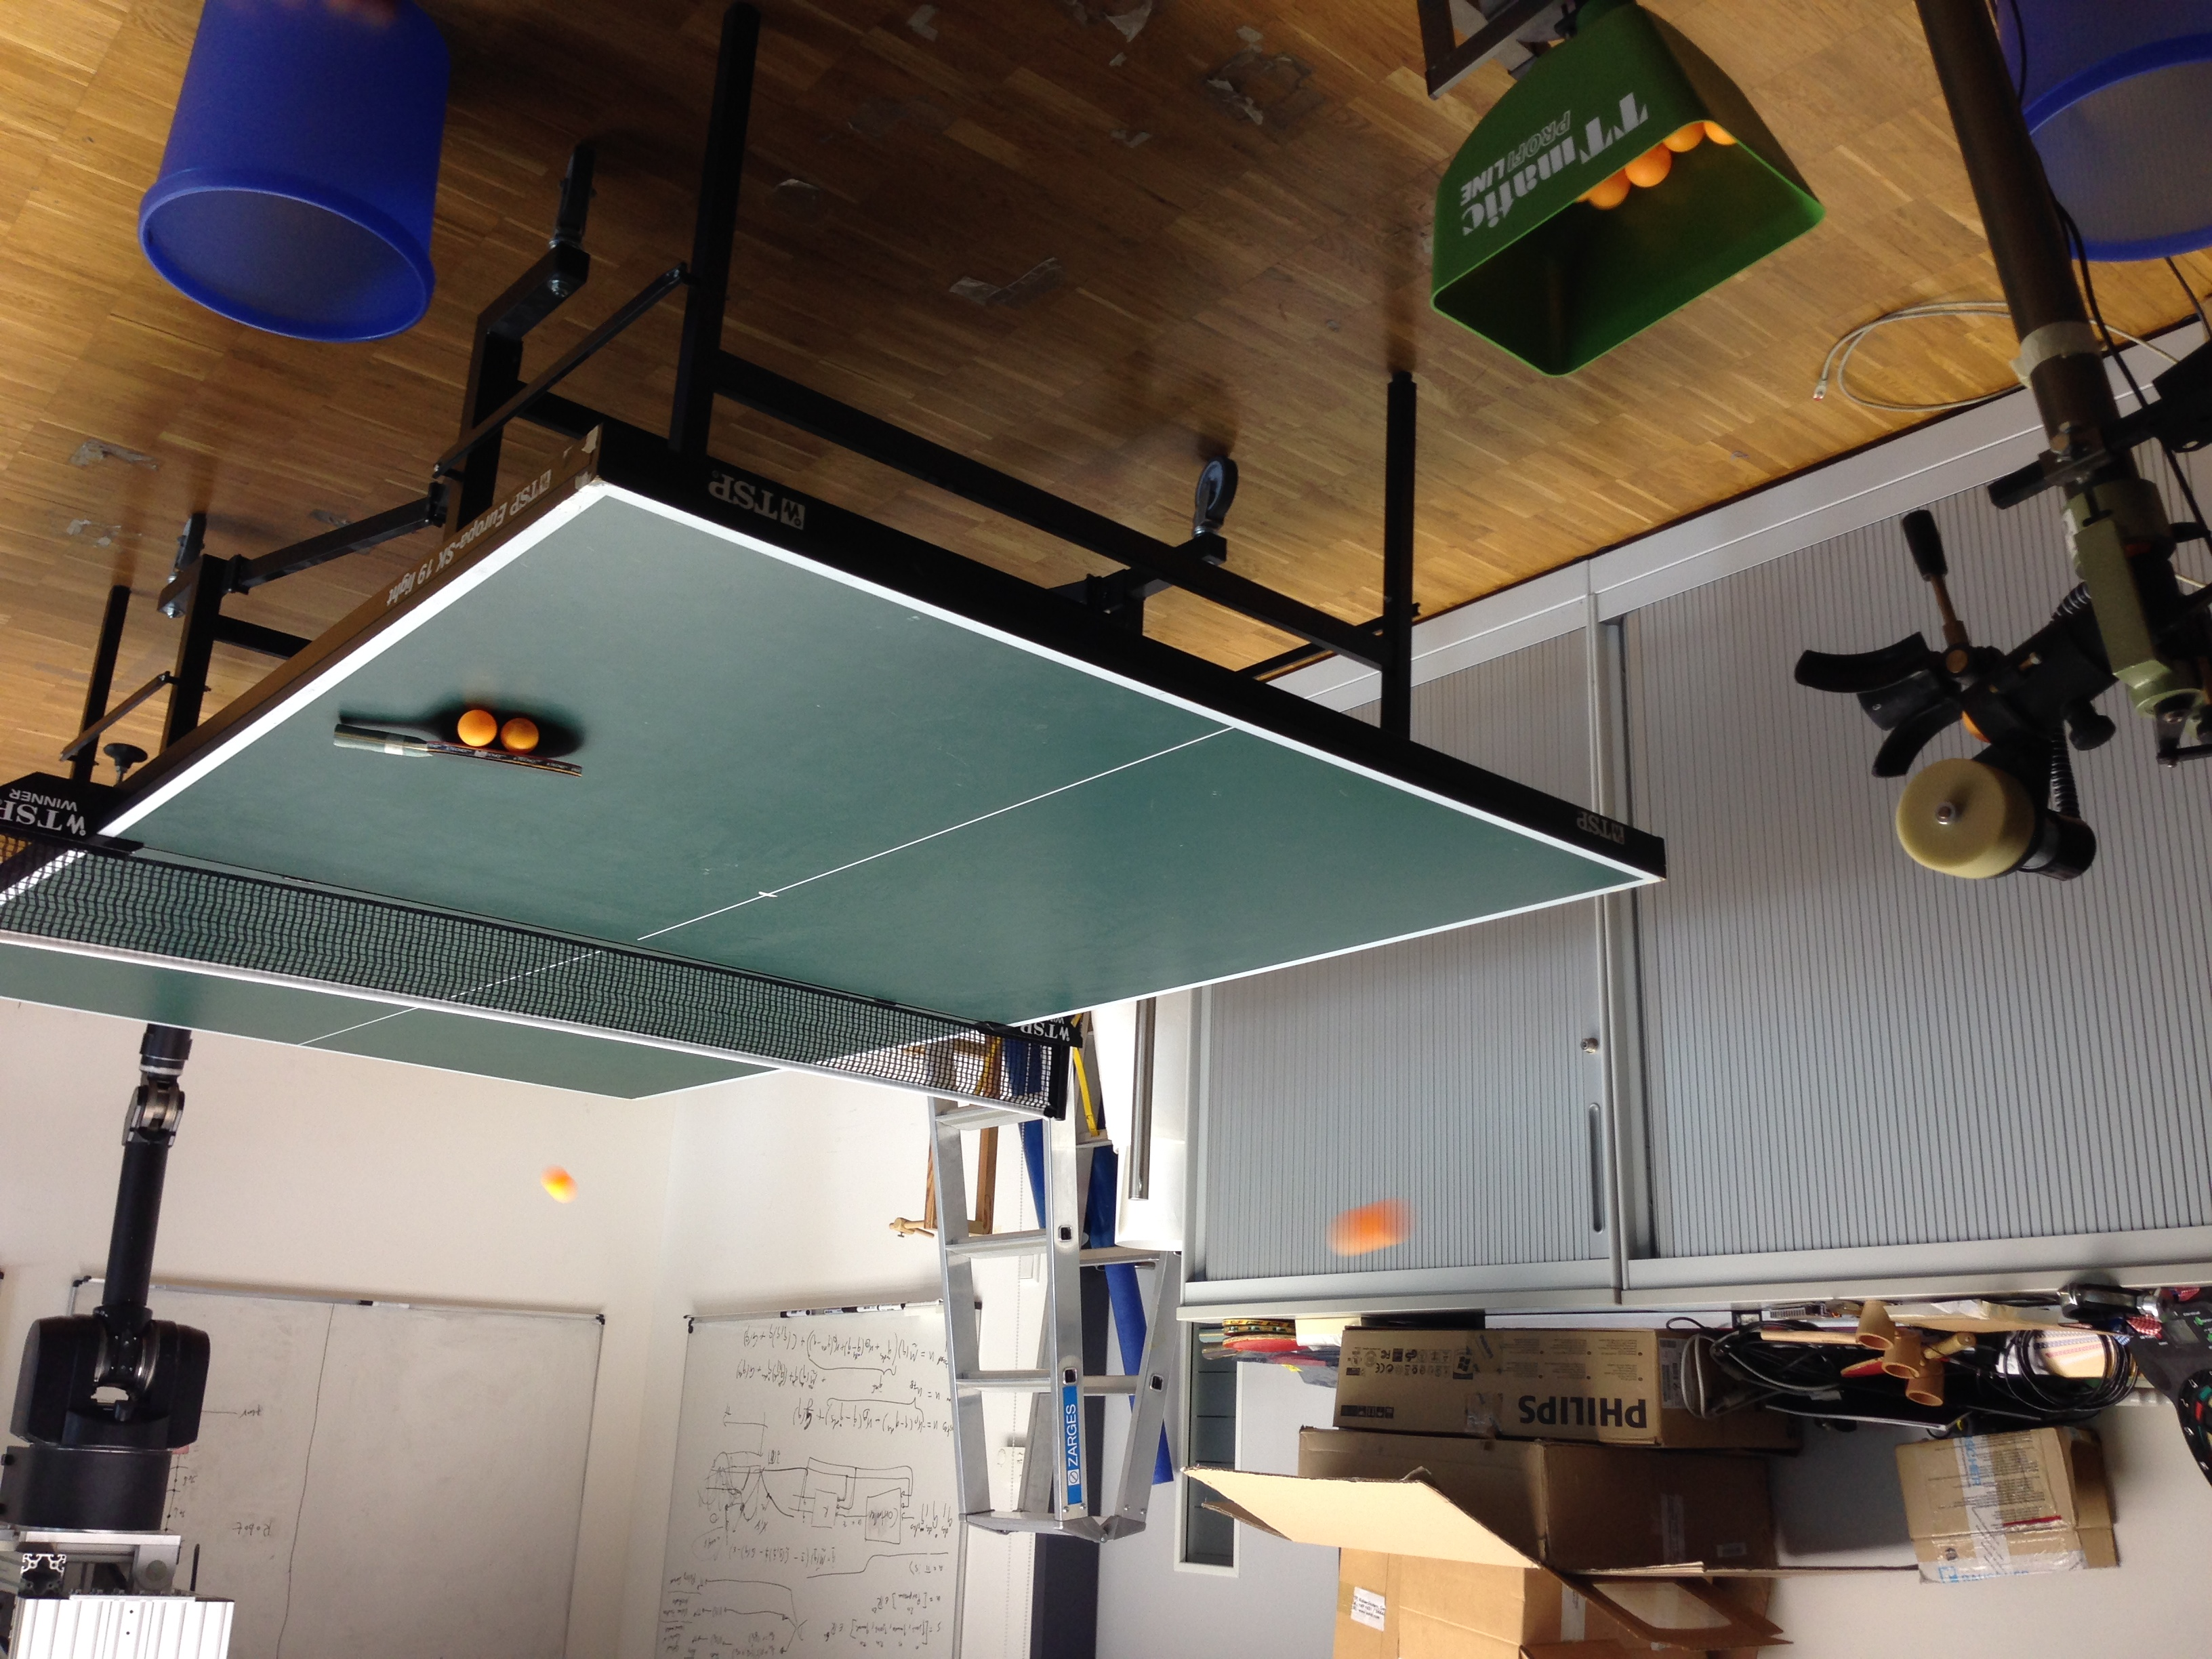
\includegraphics[scale=0.05, angle= 180]{ballgun.jpg}			
\caption{Robotic table tennis setup with the ballgun throwing balls to the robot}
\end{figure}

\section{Conclusion}

\bibliographystyle{plain}
%\bibliographystyle{./IEEEtran}
%\bibliography{./IEEEabrv,./iros2015Ref}
\bibliography{./iros2015Ref}

\end{document}
